\documentclass{beamer}
\setbeamertemplate{bibliography item}[text]

%Information to be included in the title page:
\title[QD Multiphysics Coupling]{Using Multilevel QD Projective Method for Solving Multigroup Neutron Transport Coupled with Heat Transfer}
\author[K. Hansen]{Kyle Hansen}
\institute[NCSU]{North Carolina State University}
\date[April 2026]{NE 511 Project Proposal\\Multiphysics of Nuclear Reactors\\2 April 2026}

\usetheme{Madrid}
\usecolortheme{beaver}

\usepackage{amsmath}
\usepackage{mathtools}
\newcommand{\norm}[1]{\left\| {#1} \right\|}
\usepackage{algpseudocode}
\usepackage{algorithm}
\usepackage{algorithmicx}
\usepackage{algpseudocode}
\usepackage{algorithm}
\usepackage{tikz}
\usetikzlibrary{tikzmark}
\usetikzlibrary{arrows.meta}
\newcommand*\Let[2]{\State{#1 $\gets$ #2}}
\algrenewcommand\algorithmicrequire{\textbf{Precondition:}}
\algrenewcommand\algorithmicensure{\textbf{Postcondition:}}

\newcommand{\ddz}{\frac{\partial}{\partial z}}
\newcommand{\p}{^\prime}


\begin{document}

\frame{\titlepage}

\section{Overview}

\begin{frame}
    \frametitle{Project Overview}
    Multilevel Nonlinar Projective method projects multigroup transport onto one-group Quasidiffusion (QD) equation for scalar flux.
    \begin{itemize}
        \item QD equation coupled to TH via implicit temperature dependence of cross sections
        \item Coupled system of GLOQD and TH solved with Newton iteration
    \end{itemize}
    Project scope:
    \begin{itemize}
        \item Implement MNP method for coupled neutron transport and TH
        \begin{itemize}
            \item Linear Discontinous Finite Element method for Transport Equation, MLOQD, and GLOQD
            \item Finite volume method for advection-diffusion TH equation
        \end{itemize}
        \item Fourier stability analysis for MNP method
    \end{itemize}
    Compare to NILO-CMFD method
\end{frame}

\begin{frame}
    \frametitle{Outline}
    \tableofcontents
\end{frame}



\begin{frame}[allowframebreaks]
    \frametitle{Problem Definition}

    \footnotesize
    \begin{subequations}\label{eq:long-form}
    \begin{gather}
        \mathcal{L}(T)\psi(\vec{r}, \hat{\Omega}, E, t) =\begin{multlined}[t]
         \mathcal{S}(T)\psi(\vec{r}, \hat{\Omega} E, t) \\
         + q(\vec{r}, \hat{\Omega}, E, t) + \sum_k\mathcal{P}_kC_k, \tag{Neutron Transport}
        \end{multlined}\\
        \frac{\partial C_k}{\partial t} = -\lambda_k C_k + \int\limits_{0}^{\infty}dE\; \beta_{k}(E)\nu(E)\Sigma_f(E)\int\limits_{4\pi}d\hat{\Omega} \psi(\vec{r}, \hat{\Omega}, E, t),\tag{Precursor Balance}\\
        \mathcal{H}T(\vec{r}) = \mathcal{Q}(T)\psi(\vec{r}, \hat{\Omega}, E, t),\tag{Heat Transfer}\\
        \Sigma_u(\vec{r}) = \Sigma_u\left(T, \phi\right)\tag{XS Temp. Dependence}
    \end{gather}
    \begin{minipage}{0.55\textwidth}
        \begin{gather}\addtocounter{equation}{3}
        \psi(\vec{r}, \Omega, E, 0) = \psi^0,\\
        T(\vec{r}, 0) = T^0,\\
         \psi(\vec{r}, \Omega, E, t) = \psi^{in},\; \hat{n}\cdot\hat{\Omega}<0, \vec{r} \in \partial \Gamma
    \end{gather}
    \end{minipage}
    \begin{minipage}{0.4\textwidth}
        \centering
        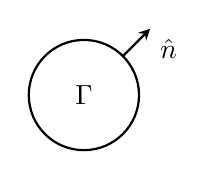
\begin{tikzpicture}[scale=0.7]
            \draw[thick] (0,0) circle (1cm);
            \node at (0,0) {$\Gamma$};
            \draw[-stealth, thick] (45:1cm) -- (45:1.7cm) node[anchor=north west] {$\hat{n}$};
        \end{tikzpicture}
    \end{minipage}
    \end{subequations} 

    \footnotesize
    \pagebreak
    \begin{subequations}
        \begin{gather}
            \mathcal{L}(T)\psi = \left[ \frac{\partial}{\partial t} + \mu \ddz  + \Sigma_t(T)  \right]\psi\\
            \mathcal{S}(T)\psi =  
            \begin{multlined}[t]
                \frac{\chi(E)}{2} \int\limits_0^\infty dE^\prime  \; \nu\Sigma_f(E^\prime, T) \int\phi(z, E^\prime, t) \\+ \frac{1}{2}\int\limits_0^\infty dE^\prime \Sigma_s(E^\prime \rightarrow E, T) \phi(z, E\p, t)
            \end{multlined}\\
            \Sigma_i = \Sigma_{i, 0} + \Sigma_{i, 1, d} \left( \sqrt{T + \beta_{fb} W_f f(z)} - \sqrt{T_{d, 0}} \right) + \Sigma_{i, 1, b}\left(T - T_0 \right) \\
            \mathcal{P}_kC_k = \frac{1}{2}\lambda_k \chi_k^{del}(z, E, t)C_k(z, t) \\
            \mathcal{Q}(T) \psi = \int\limits_{0}^\infty dE \; W_f(E)\Sigma_f(E, T)\phi(z, E, t)\\
            \mathcal{H}T = \left[ \frac{\partial}{\partial t} + \dot{m}c_p \ddz -\ddz k_b\ddz  \right]T(z)
        \end{gather}
    \end{subequations}
    \normalsize
\end{frame}


\section{Coupling Methods using CMFD}

\begin{frame}{FPI Coupling}
    \begin{alertblock}{Directly HT to High-Order Transport is expensive}
        Transport: $\vec{r}, \hat{\Omega}, E, t$

        Heat Transfer: $\vec{r}, t$
    \end{alertblock}
    \begin{figure}
        \centering
        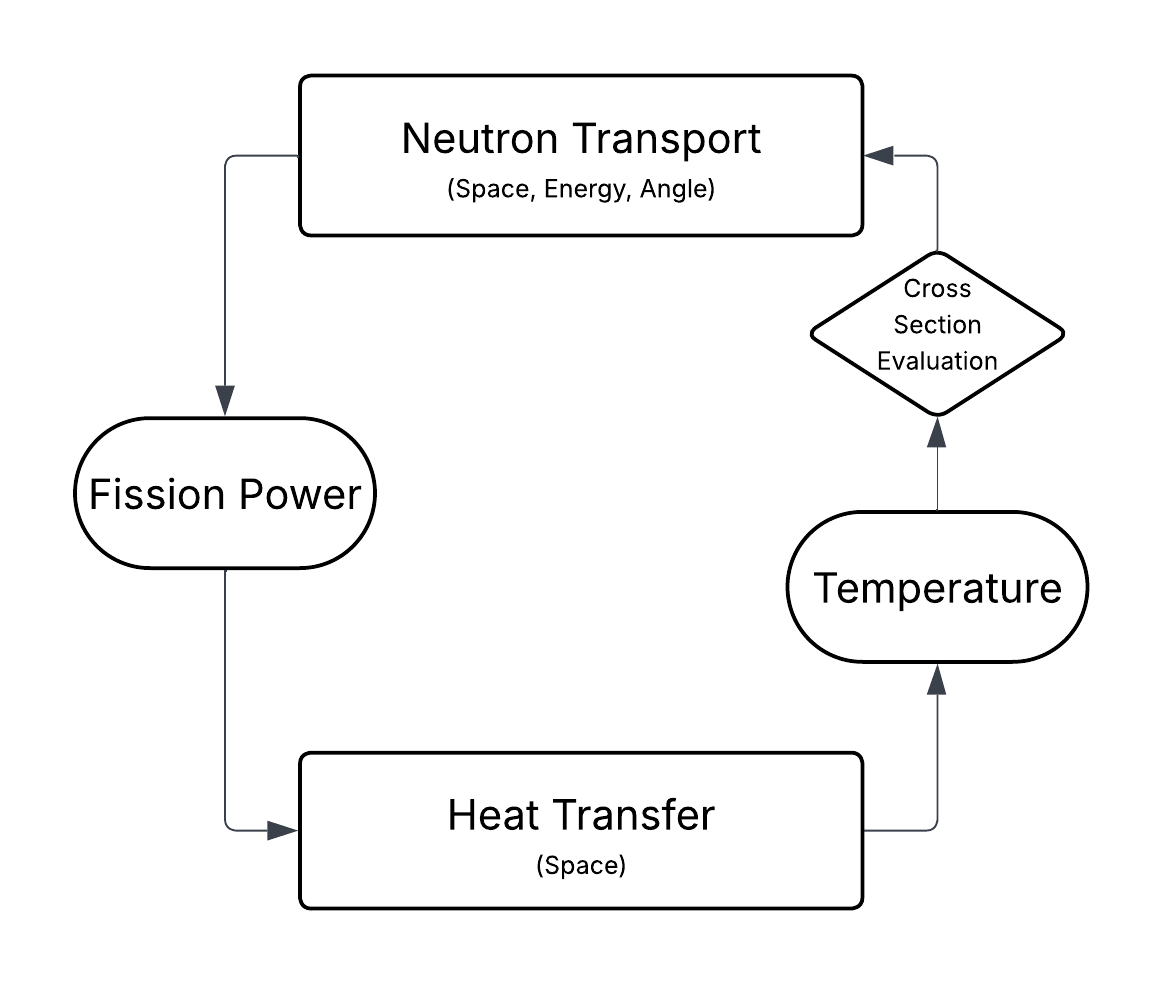
\includegraphics[width=0.6\linewidth]{images/high_order_coupling_flowchart.png}
    \end{figure}
\end{frame}

\begin{frame}{Coupling with Low-Order Operators}
    \begin{minipage}{0.6\linewidth}
        \begin{figure}
            \centering
            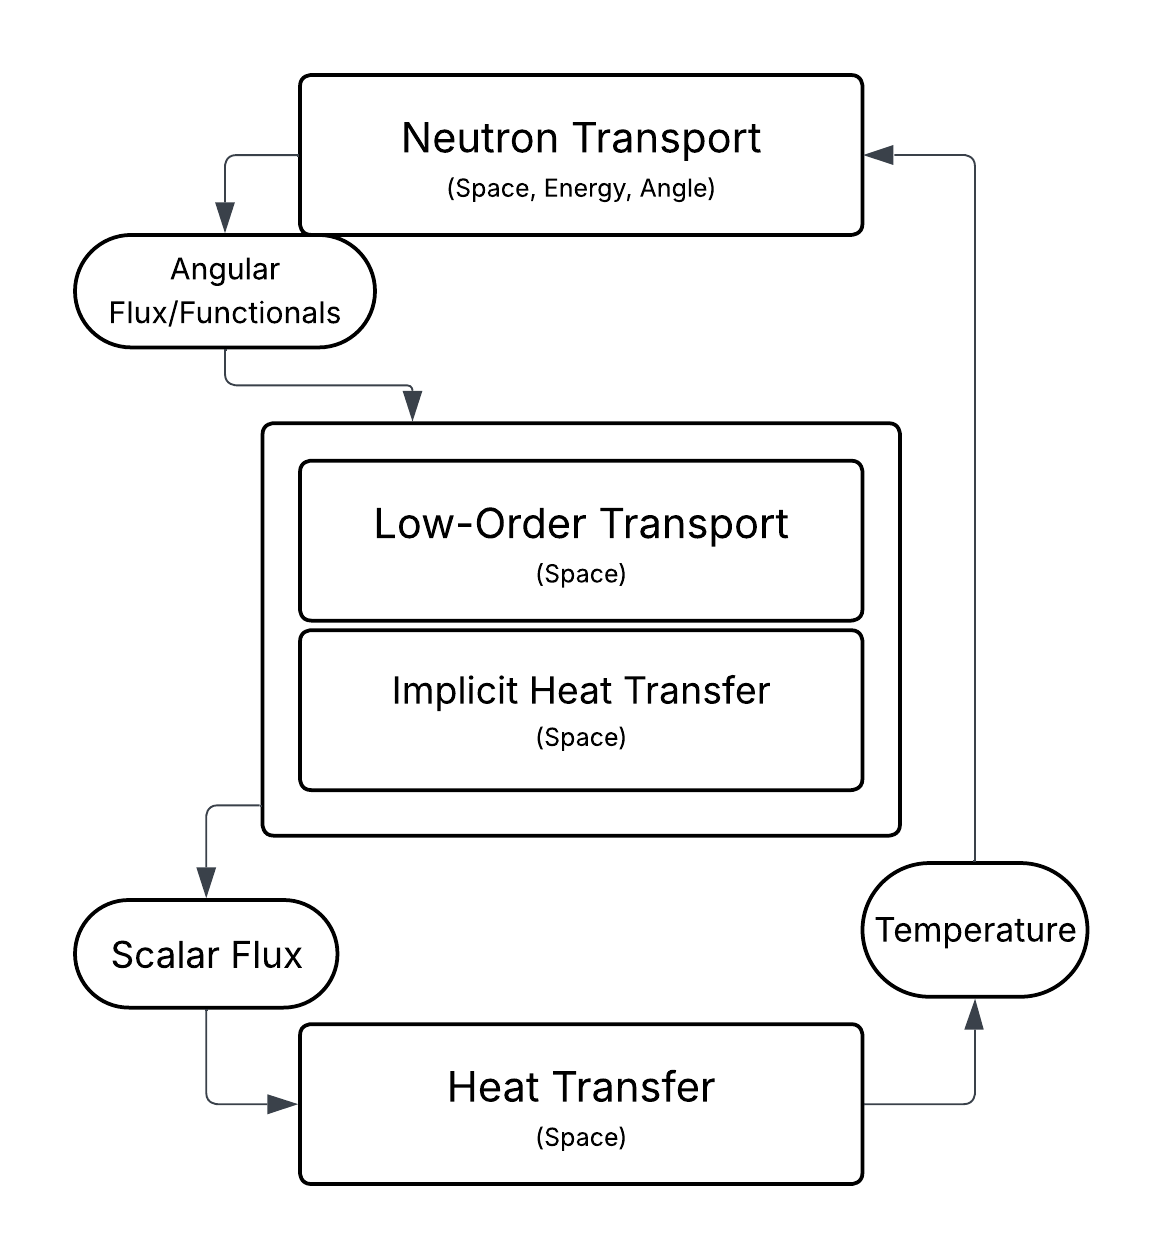
\includegraphics[width=\linewidth]{images/nilocmfd_coupling_flowchart.png}
        \end{figure}
    \end{minipage}
    \begin{minipage}{0.39\linewidth}
        \begin{itemize}
            \item Coupling is contained in LO/Approximate system
            \item Requires few solutions of NT and HT equations
            \item Can approximate TH in inner iterations without approximation in final solution
        \end{itemize}
        
    \end{minipage}
    
    
\end{frame}

\begin{frame}{CMFD Coupling Methods -- FPI-CMFD}
    CMFD aids iteration by introducing Diffusion Synthetic Acceleration (DSA) and coarse-mesh finite difference (CMFD).
    
    \vspace{1em} Most apparent coupling method: fixed-point iteration (FPI), which treats cross sections \textit{explicitly}

    \begin{gather}
        \boxed{\Sigma_i(T^n)}\tikzmarknode{arrow}{\longrightarrow}{\boxed{\mathcal{D}\phi^{(n+1)} = \mathcal{S}_{0}}} \longrightarrow  \boxed{\mathcal{H}T^{(n+1)} = \mathcal{Q}\phi^{(n+1)}}\tag{FPI}
    \end{gather}
    \begin{tikzpicture}[overlay,remember picture,black,>=Stealth, nodes={font=\small}]
        \draw[<-] (arrow) -- ++ (0, -0.5) node[below] {{$\mathcal{D}$ from transport sweep}};
\end{tikzpicture}

\begin{block}{CMFD-FPI is an Ineffective method}
    \begin{itemize}
        \item Slow to converge
        \item May be unstable
        \item Solution of HT equation is expensive
    \end{itemize}
\end{block}

\end{frame}

\begin{frame}{CMFD Coupling Methods -- R-CMFD}
    Instabilities from FPI can be resolved by ``relaxing'' the heat source on each iteration:

    \begin{gather}
        \boxed{\Sigma_i(T^n)}{\longrightarrow}{\boxed{\mathcal{D}\phi^{(n+1)} = \mathcal{S}_{0}}} \longrightarrow  \boxed{\mathcal{H}T^{(n+1)} = \mathcal{Q}(\alpha\phi^{(n+1)} + (1-\alpha)\phi^{(n)})}\tag{R-CMFD}
    \end{gather}

    R-CMFD still has its problems
    \begin{itemize}
        \item Slower to converge than FPI -- requires more HT evaluations
        \item Still may be unstable
    \end{itemize}

    
\end{frame}

\begin{frame}{CMFD Coupling Methods -- X-CMFD}
    Use implicit cross sections in low-order diffusion calculation
    
    \begin{itemize}
        \item Diffusion uses end-of-iteration xs
    \end{itemize}

    \begin{equation}
        \boxed{\mathcal{L}\psi^{(n+1)} = \mathcal{S}\phi^{(n)}}{\longrightarrow}\boxed{\begin{array}{c}
            \mathcal{D}(T^{(n+1)})\phi^{(n+1)} = \mathcal{S}_{0}\\
            \mathcal{H}T^{(n+1)} \tikzmarknode{inner}= \mathcal{Q}\phi^{(n+1)}
        \end{array}}\tag{X-CMFD}
    \end{equation}
    \begin{tikzpicture}[overlay,remember picture,black,>=Stealth, nodes={font=\footnotesize}]
        \draw (inner)  ++ (0, -0.30) node[below] {{Solved by ``inner iteration''}};
    \end{tikzpicture}

    X-CMFD addresses stability
    \begin{itemize}
        \item Stable, converges in same number of outer iterations as single-physics transport
        \item Requires repeated (expensive) solution of HT
    \end{itemize}

\end{frame}

\begin{frame}{CMFD Coupling Methods -- NILO-CMFD~\cite{adamowicz2023nilo}}
    Reduce cost of implicit solution of coupled low-order diffusion and HT
    \begin{itemize}
        \item Use approximation $H \approx \mathcal{H}$ of HT operator to update implicit cross sections within inner iterations
        \item Update cross sections by Taylor expansion (rather than table lookup or function evaluation)
    \end{itemize}

    Implicit cross section update performed during inner iterations:
    \begin{align}
        \Sigma^{(n+1)} &= \Sigma(T^{(n+1)}, h^{(n+1)})\\
                       &\approx \Sigma_i^{(n)} + \frac{\partial\Sigma}{\partial T}^{(n)}\left( T^{(n+1)} - T^{(n)} \right) + \frac{\partial \Sigma}{\partial h}\left(h^{(n+1)} - h^{(n)} \right)\\
                       &\approx \begin{multlined}[t]
                        \Sigma_i^{(n)} + \frac{\partial\Sigma}{\partial T}^{(n)}H^{-1}W\left( \Sigma_f\phi^{(n+1)} -\Sigma_f\phi^{(n)}\right)\\
                        + \frac{\partial \Sigma}{\partial h}^{(n)}W\left( \Sigma_f\phi^{(n+1)} -\Sigma_f\phi^{(n)}\right)
                       \end{multlined}
    \end{align}
\end{frame}

\section{Multilevel Low-Order Quasidiffusion}


\begin{frame}{Multigroup Low-Order Quasidiffusion}

    Take zeroth and first angular moments of the high-order multigroup NTE in 1D slab geometry

    \begin{subequations}
        \begin{multline}
            \frac{1}{v_g}\frac{\partial \phi_g}{\partial t} + \frac{\partial J_g}{\partial x} + (\Sigma_{t, g} - \Sigma_{s, g\rightarrow g})\phi_g \\
            = \sum_{g^\prime = 1}^{g-1} \Sigma_{s, g^\prime \rightarrow g}\phi_{g^\prime} + \left( Q_{s, g, 0} + \chi_g^p \overline{(1 - \beta)\nu\Sigma_f} \right)\phi + q_{del, g}^\chi
        \end{multline}
        \begin{equation}
            \frac{1}{v_g}\frac{\partial J_g}{\partial t} + \frac{\partial}{\partial x} (E_g \phi_g) + \Sigma_{t, g}J_{g} =0
        \end{equation}
        \begin{gather}
            \phi_g(x, 0) = \phi_g^0, \quad J_g(0, x) = J_g^0\\
            J_g(0, t) = C_{0, g}\phi_g(0, t), \quad J_g(X, t) = C_{X, g}\phi_g(X, t)
        \end{gather}
    \end{subequations}

    
\end{frame}

\begin{frame}{Closure terms}
    QD equations and high-order equations closed by Eddington and boundary factors:

    \begin{equation}
        E_g = \frac{\int_{-1}^{1}d\mu\, \mu^2 \psi_g}{\int_{-1}^{1}d\mu\, \psi_g},
    \end{equation}
    \begin{equation}
        B_{0, g} = \frac{\int_{-1}^{0}d\mu\, \mu\psi_{g}(0, \mu)}{\int_{-1}^{0}d\mu\, \psi_{g}(0, \mu)}, \qquad B_{X, g} = \frac{\int_{0}^{1}d\mu\, \mu\psi_{g}(X, \mu)}{\int_{0}^{1}d\mu\, \psi_{g}(X, \mu)}
    \end{equation}
\end{frame}

\begin{frame}{Grey Low-Order Quasidiffusion (GLOQD)}
    Sum the Multigroup LOQD equations to yield

    \begin{subequations}
        \begin{equation}
            \frac{\partial}{\partial t} \left(\frac{\phi}{\overline{v}} \right) + \frac{\partial J}{\partial x} + \left( \overline{\Sigma}_a + \overline{(1-\beta)\nu\Sigma_f}\right)\phi = q_{del}^\chi
        \end{equation}
        \begin{equation}
            \frac{\partial}{\partial t}\left( \frac{J}{\hat{v}} \right) + \frac{\partial}{\partial x} \left( \overline{E}\phi\right) + \overline{\Sigma}_{tr}J + \overline{\zeta}\phi = 0
        \end{equation}
        \begin{gather}
            \phi(x, 0) = \phi^0, \quad J(x, 0) = J^0,\\
            J(0, t) = \overline{B}_{0}\phi(0, t), \quad J(X, t) = \overline{B}_X\phi(X, t)
        \end{gather}
    \end{subequations}

    \begin{block}{Effect of projection}
        \centering
        High-order NTE $\longrightarrow$ MLOQD $\longrightarrow$ GLOQD
        \[ (x, \mu, E, t) \longrightarrow  (x, E, t)  \longrightarrow (x,t)\]
        Project NTE to same dimensionality as HT
    \end{block}
\end{frame}



\section{Project Scope}

\begin{frame}{General Project Goals}
    Combine Advantages of NILO-CMFD~\cite{adamowicz2023nilo} and MLOQD~\cite{tamang2014multilevel}, write my own implementation

    \begin{itemize}
        \item Couple NTE and HT using Nonlinearly Implicit Low-Order coupling and Multigroup Low-Order Quasidiffusion
        \item Consider delayed neutrons (not included in CMFD results)
        \item 1D slab geometry, Linear Discontinuous (LD) finite element method
        \item HT: advection-diffusion equation using finite volume method
    \end{itemize}

    Perform Fourier stability analysis of NILO-MLOQD method
    \begin{itemize}
        \item Ensure stability for all parameters
        \item Estimate performance of method (iterations saved)
        \item Compare Fourier results with numerical results
    \end{itemize}
    
\end{frame}



\begin{frame}{Time, spatial, and angular discretization of ELOT problem}
    Consider 1D slab/channel geometry with isotropic scattering. Discretize transport using
    % \small
    \begin{itemize}
        \item Angle -- Discrete Ordinates
        \item Time -- Backward Euler
        \item Space -- LD Galerkin Method
    \end{itemize}
    
    and discretize HT using Finite Volume method.

    I will implement in Python, but can be scaled up to 2/3D using tools such as MFEM~\cite{anderson2021mfem}

    \begin{figure}
        \centering
        \tiny
        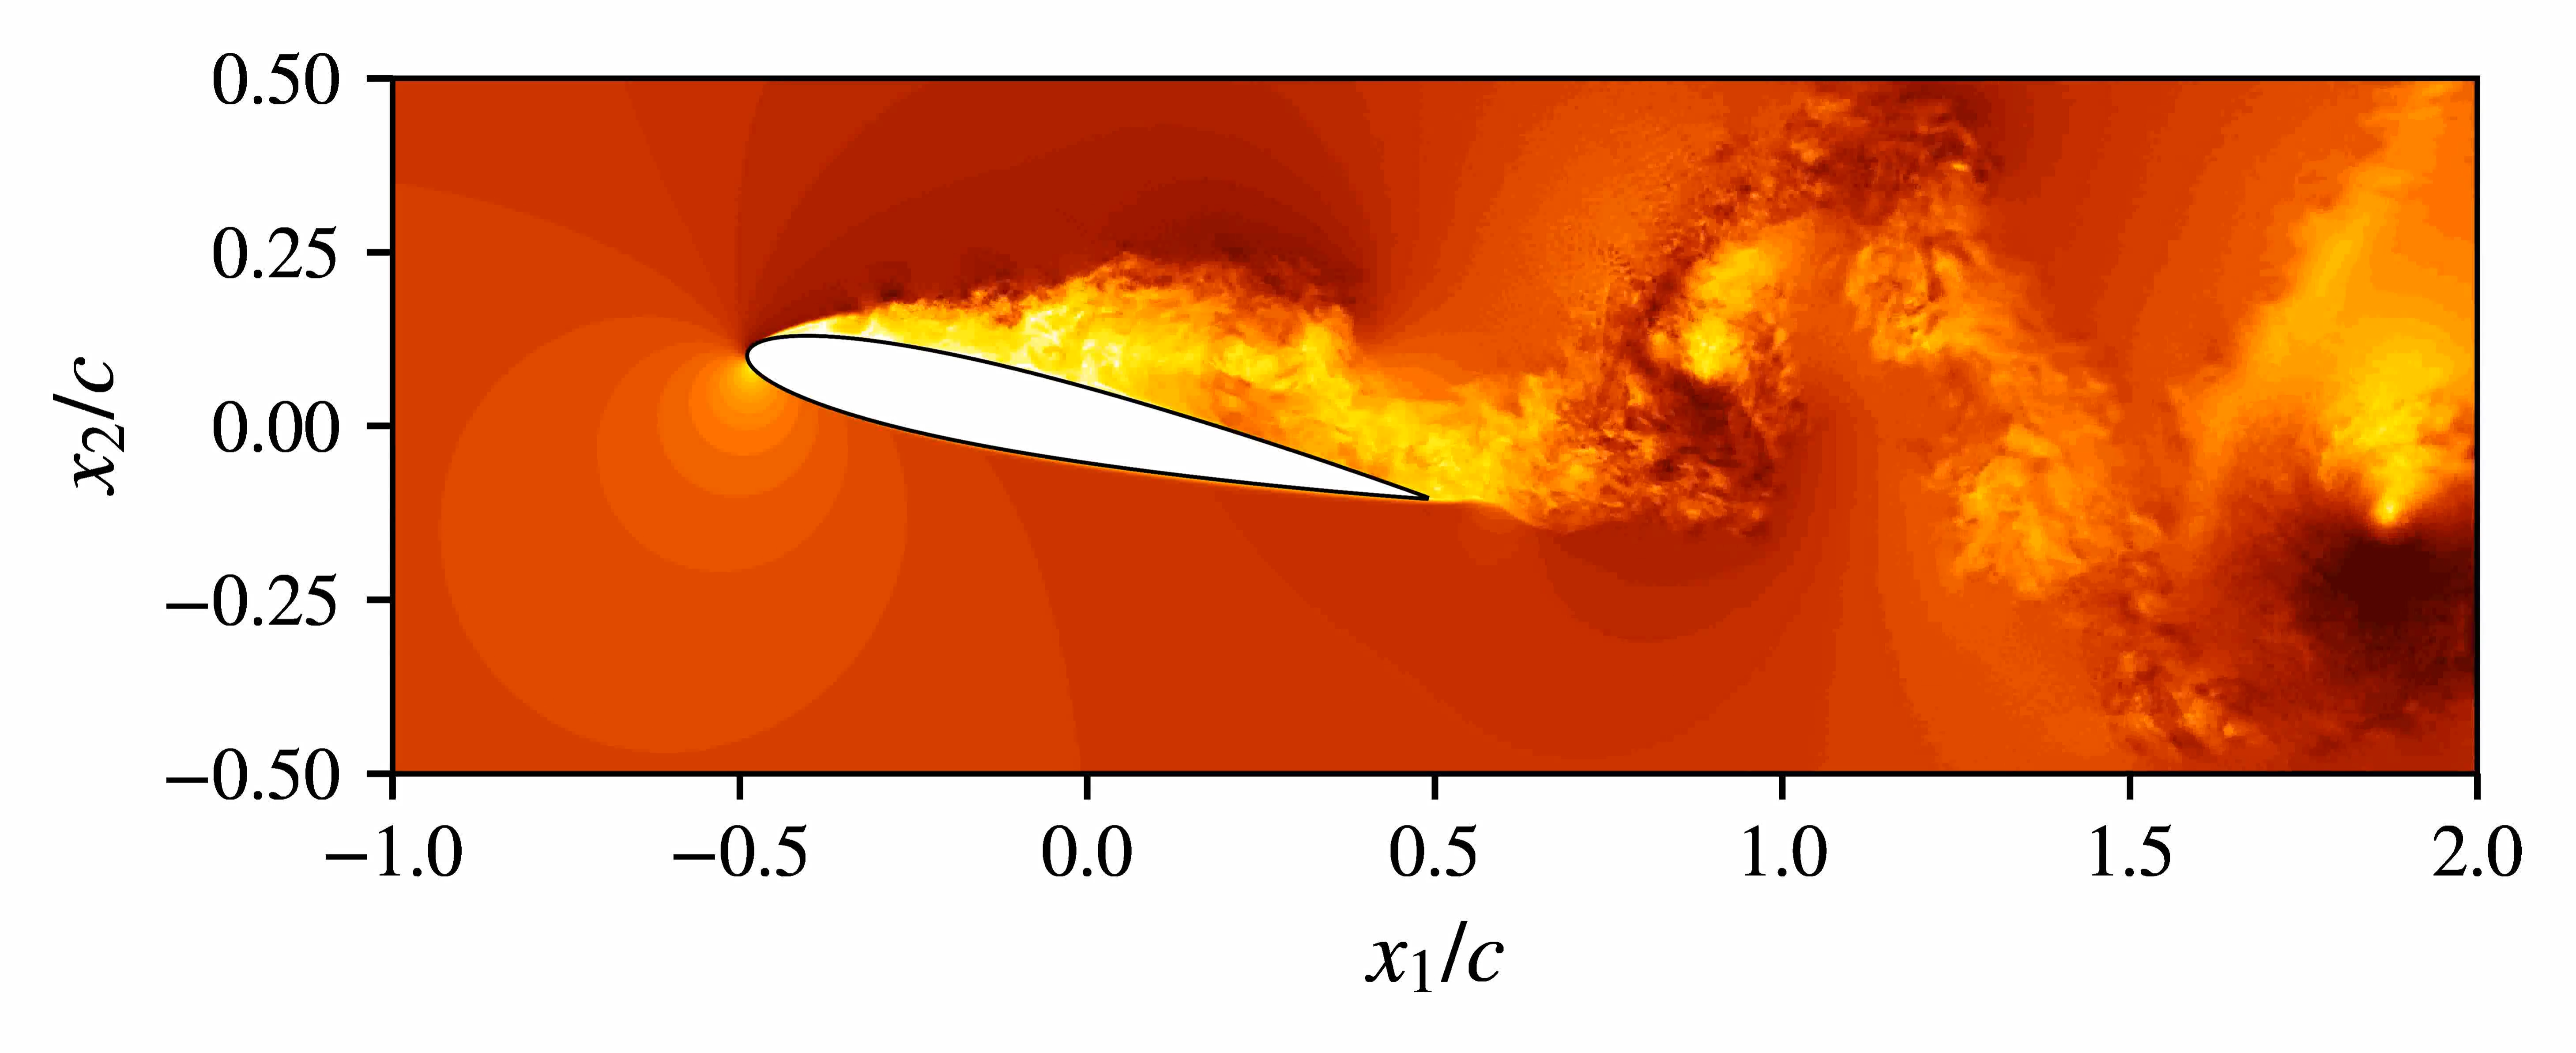
\includegraphics[width=0.6\linewidth]{images/mfem_demo.png}
        
        MFEM Navier Minapp (Spieser 2023)
    \end{figure}



\end{frame}









\begin{frame}[allowframebreaks]
    \frametitle{References}
    \bibliographystyle{ieeetr}
    \bibliography{references.bib}
\end{frame}


\end{document} 